\documentclass[fontsize=11pt]{scrartcl}
\usepackage[T1]{fontenc}
\usepackage{fourier}

\usepackage[english]{babel}                                                         % English language/hyphenation
\usepackage[protrusion=true,expansion=true]{microtype}  
\usepackage{amsmath,amsfonts,amsthm} % Math packages
\usepackage[pdftex]{graphicx}   
\usepackage{url}
\usepackage{listings}

%%% Custom sectioning
\usepackage{sectsty}
\allsectionsfont{\centering \normalfont\scshape}


%%% Custom headers/footers (fancyhdr package)
\usepackage{fancyhdr}
\pagestyle{fancyplain}
\fancyhead{}                                            % No page header
\fancyfoot[L]{}                                         % Empty 
\fancyfoot[C]{}                                         % Empty
\fancyfoot[R]{\thepage}                                 % Pagenumbering
\renewcommand{\headrulewidth}{0pt}          % Remove header underlines
\renewcommand{\footrulewidth}{0pt}              % Remove footer underlines
\setlength{\headheight}{13.6pt}


%%% Equation and float numbering
\numberwithin{equation}{section}        % Equationnumbering: section.eq#
\numberwithin{figure}{section}          % Figurenumbering: section.fig#
\numberwithin{table}{section}               % Tablenumbering: section.tab#


%%% Maketitle metadata
\newcommand{\horrule}[1]{\rule{\linewidth}{#1}}     % Horizontal rule

\title{
        %\vspace{-1in}  
        \usefont{OT1}{bch}{b}{n}
        \horrule{0.5pt} \\[0.4cm]
        \huge Optimizing Single Core Matrix Multiply \\
        \horrule{2pt} \\[0.5cm]
}
\author{
        \normalfont                                 \normalsize
        Group 2\\[-3pt]      \normalsize
        \today
}
\date{}


%%% Begin document
\begin{document}

\maketitle

\section{Intro}
Matrix multiplication is a ubiquitous operation in science and engineering,
and thus the efficient and fast computation of matrix products is essential.
This report serves as an initial report into tuning the performance of matrix
multiplication on a single core.

\subsection{Matrix Multiplication}
Throughout this report, we will consider the problem of computing
$C = A B$, where $C, A, B$ are $M \times M$ square matrices.

\begin{lstlisting}[frame = single, caption={Naive Square Matrix Multiply}]
void square dgemm(const int M, 
                  const double *A, const double *B, double *C)
{
    for (int i = 0; i < M; ++i) {
        for (int j = 0; j < M; ++j) {
            for (int k = 0; k < M; ++k) {
                C[j*M+i] += A[k*M+i] * B[j*M+k];
            }
        }
    }
}
\end{lstlisting}

\subsection{Testing specs}

\section{Optimization strategies}

At this time, two different optimization strategies have been implemented and
tested: reorganizing the loops to restructure the order of computation, and 
partitioning matrix into sub-blocks, in order to promote cache reuse.

\subsection{Loop ordering}
Notice that in the naive matrix multiply implementation, the innermost loop
is where all the work is done.  Thus, the order of the loops does not matter.
Noting this, we can choose the loop order that best regularizes memory access.
Ideally, we would like to access the arrays with stride 1, and this motivates the
idea that the `i' variable in the above naive code should be looped over in the 
innermost loop, as then we are accessing C and A with stride one.  This results in 
the following code:

\begin{lstlisting}[frame = single, caption={Improved Loop Order Square Matrix Multiply}]
void square dgemm(const int M, 
                  const double *A, const double *B, double *C)
{
    for (int j = 0; j < M; ++j) {
        for (int k = 0; k < M; ++k) {
            double bkj = B[j*M+k];
            for (int i = 0; i < M; ++i)
                C[j*M+i] += A[k*M+i] * bkj;
        }
    }
}
\end{lstlisting}

This optimization is supported empirically, as all possible loop orders were
tested (see Figure~\ref{fig:loop_order}).

This basic optimization brings the naive matrix multiple up to the speed of
the provided Fortran code (see Figure~\ref{fig:loop_order_opt_comparison}).

\begin{figure}
    \centering
    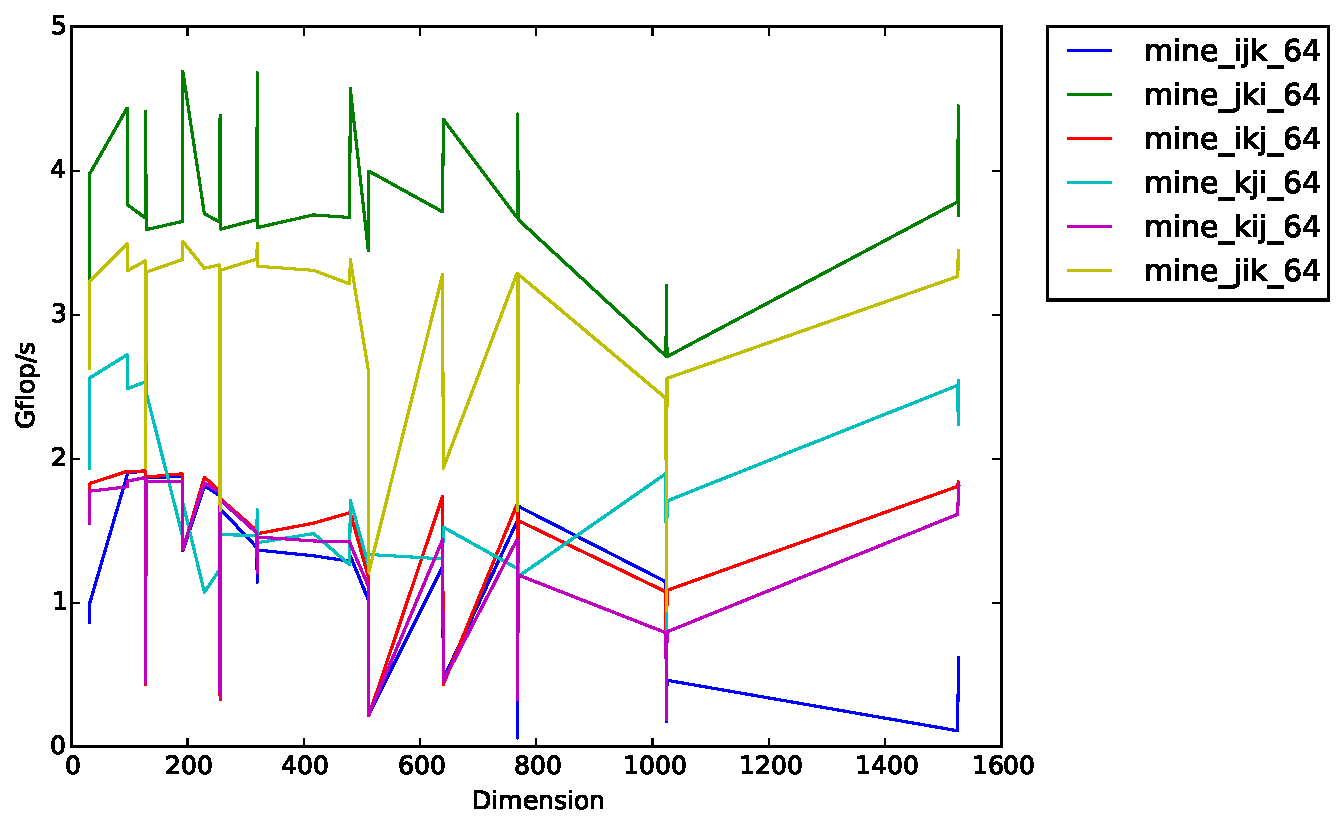
\includegraphics[width=6.0in]{../timings/timings loop order.pdf}
    \caption{Results for all possible loop orders}
    \label{fig:loop_order}
\end{figure}

\begin{figure}
    \centering
    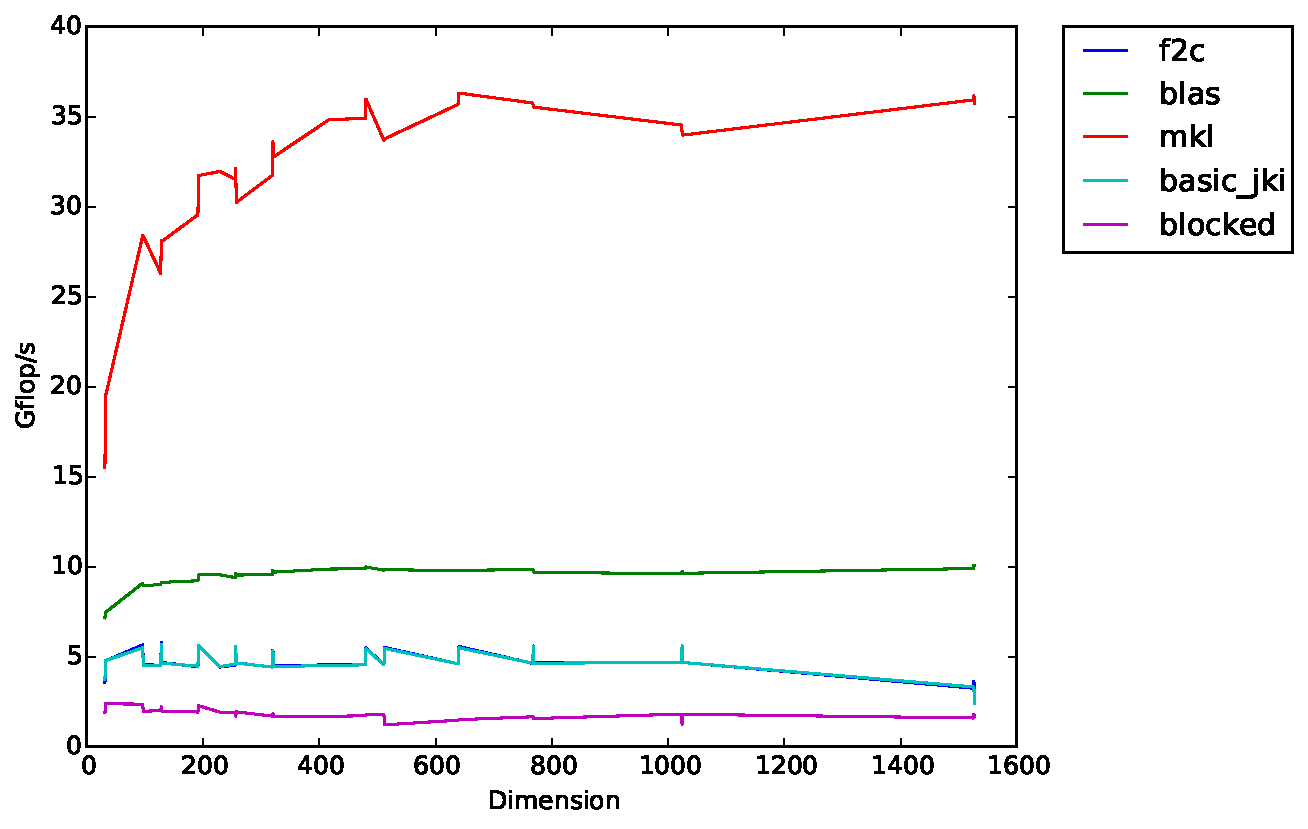
\includegraphics[width=6.0in]{../timings/timing show jki good.pdf}
    \caption{Loop order optimization comparison}
    \label{fig:loop_order_opt_comparison}
\end{figure}

\subsection{Block and Copy Optimization}
In order to encourage cache reuse, and thus reducing the overhead of loading 
data from main memory when performing the floating point operations, it may make
sense to partition the matrices into sub-matrices.  All possible sub-matrix pairs
from $A$ and $B$ can then be multiplied together independently, and the resulting
sub-matrix added to the appropriate memory locations for $C$.  The scheme can be 
applied recursively to partition into sub-sub-matrices and so on.

Our current implementation is to divide the matrices $A, B, C$ into square sub-matrices
of fixed size.  We then copy the values from these sub-matrices into temporary working
arrays of aligned memory.  These sub-matrices are then further divided into sub-sub-matrices
of size $8 \times 8$.  These $8 \times 8$ matrices are then multiplied together with an 
optimized loop that can take advantage of vectorization.

Tuning this implementation is still ongoing.  Currently a good sub-matrix size seems
to be $96 \times 96$, but this barely outperforms the naive unblocked method with 
optimized loop order.  

\section{Future Work}

To further tune our matrix multiplication routine, we will continue to work on the 
blocking strategy so that we can hopefully significantly outperform an unblocked routine.
Exploring compiler optimization options will also hopefully lead to speedups.

%%% End document
\end{document}